\documentclass[tikz,border=10pt]{standalone}
\usepackage{tkz-graph}
\usepackage{amsmath,amssymb}
\usepackage{xcolor}
\usetikzlibrary{calc}
\usetikzlibrary{positioning}
\usetikzlibrary{arrows.meta}
\usetikzlibrary{decorations.pathreplacing}
\usepackage{listofitems} % for \readlist to create arrays

\definecolor{mymauve}{rgb}{0.58,0,0.82}
\definecolor{mygold}{HTML}{B8860B}
\definecolor{mynavy}{HTML}{000080}
\definecolor{olivegreen}{rgb}{0,0.6,0}

\colorlet{myred}{red!80!black}
\colorlet{myblue}{blue!80!black}
\colorlet{mygreen}{green!60!black}
\colorlet{myorange}{orange!70!red!60!black}
\colorlet{mydarkred}{red!30!black}
\colorlet{mydarkblue}{blue!40!black}
\colorlet{mydarkgreen}{green!30!black}




\begin{document}


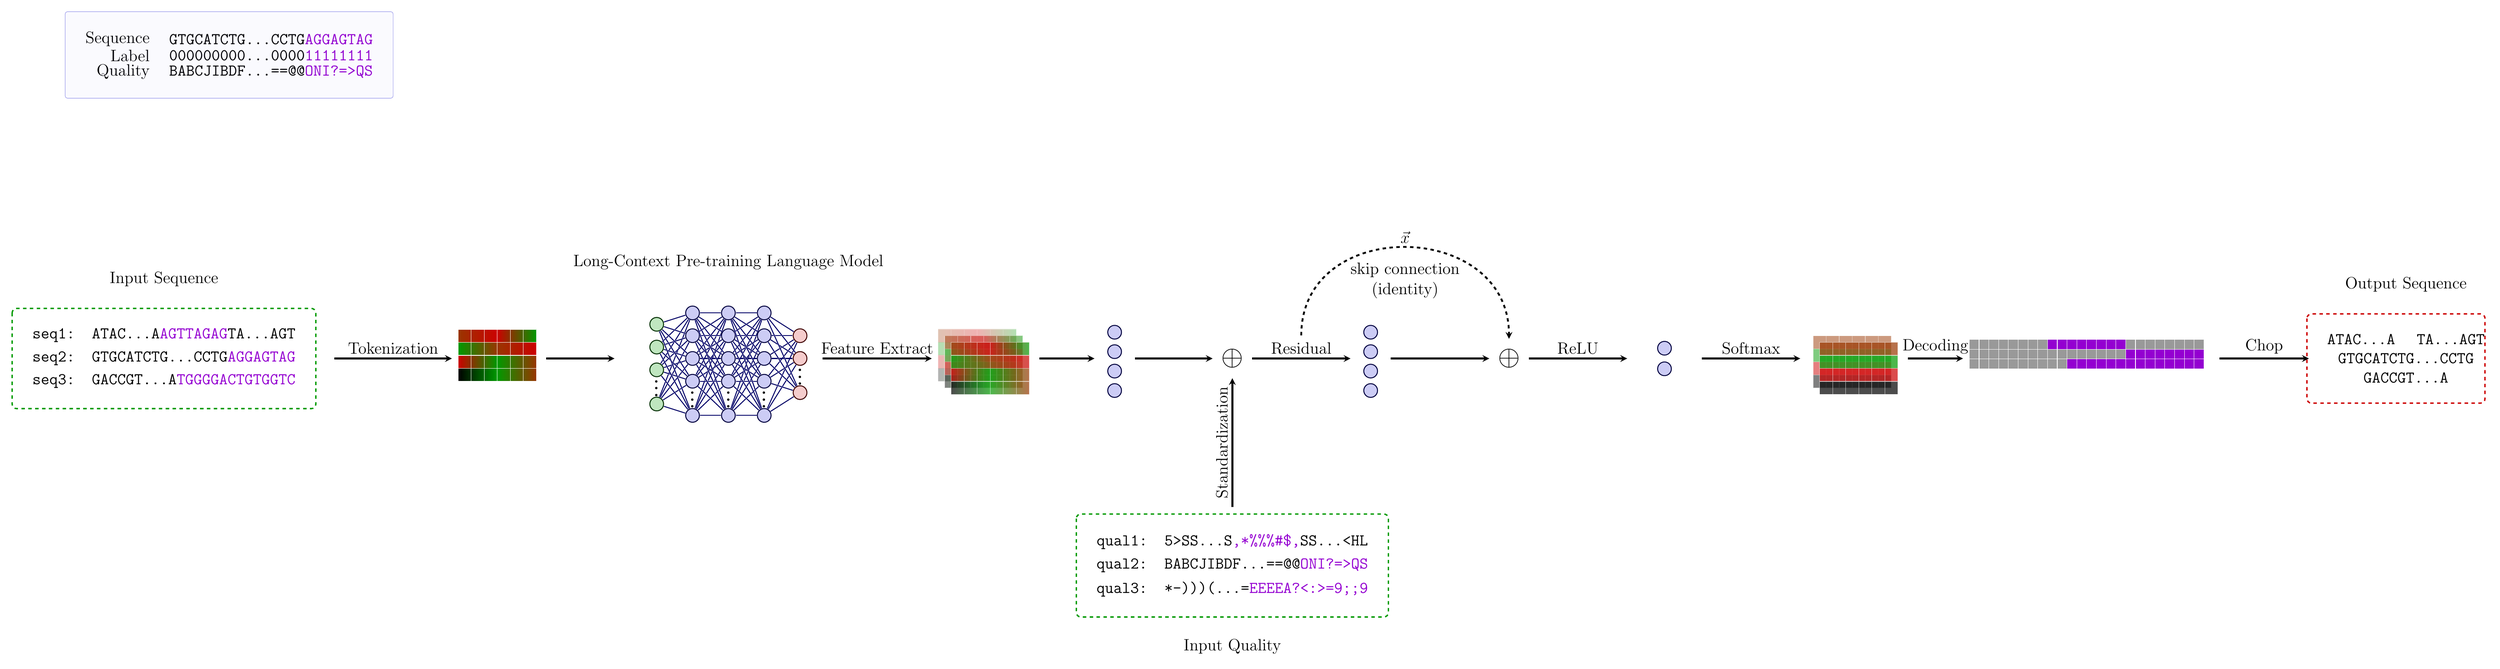
\begin{tikzpicture}[
		node/.style={thick,circle,draw=myblue,minimum size=12, inner sep=0.5,outer sep=0.6},
		node in/.style={node,green!20!black,draw=mygreen!30!black,fill=mygreen!25},
		node hidden/.style={
				node,
				blue!20!black,
				draw=myblue!30!black,
				fill=myblue!20,
			},
		node out/.style={node,red!20!black,draw=myred!30!black,fill=myred!20},
		connect/.style={-stealth, ultra thick, shorten <=2pt, shorten >=2pt},
		every node/.style={font=\Large}
	]

	\begin{scope}[scale=1, local bounding box=seqbox]
		\node (seq) at (0,0) {\tt GTGCATCTG\dots CCTG\textcolor{mymauve}{AGGAGTAG}};
		\node (label) at (0,-0.5) {\tt 000000000\dots 0000\textcolor{mymauve}{11111111}};
		\node (qual) at (0,-1) {\tt BABCJIBDF\dots ==@@\textcolor{mymauve}{ONI?=>QS}};

		% add name seq and label to the left part of the sequence
		\node[left = 1em of seq] (seq_text)  {Sequence};
		\node[left = 1em of label]  (label_text) {Label};
		\node[left = 1em of qual] (qual_text)  {Quality};
		% add a box around the sequence 
		\draw [myblue!40, fill=myblue, fill opacity=0.02,rounded corners=2]  ($(seq_text.north west) + (-0.5, 0.5)$) rectangle ($(qual.south east) + (0.5, -0.5)$);
	\end{scope}


	% add model architecture                             relu     residual ----------------
	%                                                                                     | relu
	% seq -> tokenization -> embedding ->  linear layer ------> + ------> linear layer -> + -----> output
	%                                                           |
	%                                                          qual 
	\begin{scope}[shift={($(seqbox.south)+(-2,-8)$)}, scale=1, local bounding box=modelbox1]
		% define box size 
		\def\boxsize{6em}
		\def\boxdist{9em}
		\def\boxcolor{myblue}
		\def\nodedist{1.7em}

		% add seq -> tokenization
		\node (seq) at (0,0) { \tt seq2: GTGCATCTG\dots CCTG\textcolor{mymauve}{AGGAGTAG}};
		\node[below = 1pt of seq] (seq2)  { \tt seq3: GACCGT\dots A\textcolor{mymauve}{TGGGGACTGTGGTC}};
		\node[above = 1pt of seq] (seq3)  { \tt seq1: ATAC\dots A\textcolor{mymauve}{AGTTAGAG}TA\dots AGT};

		% draw a box around the sequence
		\draw[olivegreen, dashed, rounded corners, very thick] ($(seq3.north west) + (-0.5, 0.5)$) rectangle ($(seq2.south east) + (0.5, -0.5)$);
		\node[above = 3em of seq3, align=center] (seq_text) {Input Sequence};

		% Draw the edge from seq to a point to the right (formerly 'token') and label it
		\node[right = 1.5 * \boxdist of seq] (token) {}; % Define position without drawing the node
		\node[right = 1.5 * \boxdist of token] (pretrain) {};
		% add embedding as rectangle
		\node[right = 3 * \boxdist of pretrain] (embed)  {};

		% Draw the matrix directly at the position of the matrix node
		\begin{scope}[shift={(token.center)}, yshift=-2em, scale=0.4, local bounding box=token_box]
			% Draw the matrix contents as shades
			\shade[left color=myorange, right color=mygreen, middle color=myred] (0,3) rectangle ++(6,1);
			\shade[left color=mygreen, right color=myred, middle color=myorange] (0,2) rectangle ++(6,1);
			\shade[left color=myred, right color=myorange, middle color=mygreen] (0,1) rectangle ++(6,1);
			\shade[left color=black, right color=myorange, middle color=mygreen] (0,0) rectangle ++(6,1);
			\draw [white] (0,0) grid (6,4);
		\end{scope}

		% add arrow from seq to token
		\draw[connect] ($(seq.east) + (1, 0)$) -- node[midway, above] {Tokenization} (token);
		% add arrow from token to embedding
		\draw[connect] ($(token.east) + (2.5, 0)$) -- (pretrain);
		\draw[connect] ($(pretrain.east) + (6, 0)$) -- (embed) node [midway, above] {Feature Extract};

		% NEURAL NETWORK with coefficients, shifted
		\begin{scope}[shift={(pretrain)}, yshift=1em,  x=2.2cm, y=1.4cm, scale=0.5,
			local bounding box=pretrain_box,
			connect/.style={thick,mydarkblue}, %,line cap=round
			connect arrow/.style={-{Latex[length=4,width=3.5]},thick,mydarkblue,shorten <=0.5,shorten >=1},
			node 1/.style={node in}, % node styles, numbered for easy mapping with \nstyle
			node 2/.style={node hidden},
			node 3/.style={node out}
			]
			\def\nstyle{int(\lay<\Nnodlen?min(2,\lay):3)} % map layer number onto 1, 2, or 3

			\message{^^JNeural network, shifted}
			\readlist\Nnod{4,5,5,5,3} % array of number of nodes per layer
			\readlist\Nstr{n,m,m,m,k} % array of string number of nodes per layer
			\readlist\Cstr{\strut x,a^{(\prev)},a^{(\prev)},a^{(\prev)},y} % array of coefficient symbol per layer
			\def\yshift{0.5} % shift last node for dots

			\message{^^J  Layer}
			\foreachitem \N \in \Nnod{ % loop over layers
				\def\lay{\Ncnt} % alias of index of current layer
				\pgfmathsetmacro\prev{int(\Ncnt-1)} % number of previous layer
				\message{\lay,}
				\foreach \i [evaluate={\c=int(\i==\N); \y=\N/2-\i-\c*\yshift;
							\index=(\i<\N?int(\i):"\Nstr[\lay]");
							\x=\lay; \n=\nstyle;}] in {1,...,\N}{ % loop over nodes
						% NODES
						\node[node \n] (N\lay-\i) at (\x,\y) {};

						% CONNECTIONS
						\ifnum\lay>1 % connect to previous layer
							\foreach \j in {1,...,\Nnod[\prev]}{ % loop over nodes in previous layer
									\draw[connect,white,line width=1.2] (N\prev-\j) -- (N\lay-\i);
									\draw[connect] (N\prev-\j) -- (N\lay-\i);
									%\draw[connect] (N\prev-\j.0) -- (N\lay-\i.180); % connect to left
								}
						\fi % else: nothing to connect first layer

					}
				\path (N\lay-\N) --++ (0,1+\yshift) node[midway,scale=1.5] {$\vdots$};
			}
		\end{scope}

		\node[above=  of pretrain_box, align=center] (nn_text) {Long-Context Pre-training Language Model};

		\begin{scope}[shift={(embed.center)},yshift=-2em, scale=0.4, local bounding box=embed_box]
			\begin{scope}[opacity=0.3]
				\shade[left color=myorange, right color=mygreen, middle color=myred] (0,3) rectangle ++(6,1);
				\shade[left color=mygreen, right color=myred, middle color=myorange] (0,2) rectangle ++(6,1);
				\shade[left color=myred, right color=myorange, middle color=mygreen] (0,1) rectangle ++(6,1);
				\shade[left color=black, right color=myorange, middle color=mygreen] (0,0) rectangle ++(6,1);
				\draw [white] (0,0) grid (6,4);
			\end{scope}

			\begin{scope}[shift={(0.5, -0.5)}, opacity=0.5]
				\shade[left color=myorange, right color=mygreen, middle color=myred] (0,3) rectangle ++(6,1);
				\shade[left color=mygreen, right color=myred, middle color=myorange] (0,2) rectangle ++(6,1);
				\shade[left color=myred, right color=myorange, middle color=mygreen] (0,1) rectangle ++(6,1);
				\shade[left color=black, right color=myorange, middle color=mygreen] (0,0) rectangle ++(6,1);
				\draw [white] (0,0) grid (6,4);
			\end{scope}

			\begin{scope}[shift={(1, -1)}, opacity=0.7]
				\shade[left color=myorange, right color=mygreen, middle color=myred] (0,3) rectangle ++(6,1);
				\shade[left color=mygreen, right color=myred, middle color=myorange] (0,2) rectangle ++(6,1);
				\shade[left color=myred, right color=myorange, middle color=mygreen] (0,1) rectangle ++(6,1);
				\shade[left color=black, right color=myorange, middle color=mygreen] (0,0) rectangle ++(6,1);
				\draw [white] (0,0) grid (6,4);
			\end{scope}
		\end{scope}


		\node[\boxcolor, right = 1.5 * \boxdist of embed,  very thick, rounded corners, minimum size= 0.5 * \boxsize] (weight_layer1) {};
		\node[node hidden, yshift=  2.3em] (n1) at (weight_layer1.center) {};
		\node[node hidden, yshift={(2.3em - \nodedist)}] (n2) at (weight_layer1.center) {};
		\node[node hidden, yshift={(2.3em - 2*\nodedist)}] (n3) at (weight_layer1.center) {};
		\node[node hidden, yshift={(2.3em - 3*\nodedist)}] (n4) at (weight_layer1.center) {};


		% add a plus sign to show residual connection
		\node[right= 0.8 * \boxdist of weight_layer1, font=\Huge, minimum size= 0.5 * \boxsize] (add1) {$\oplus$};

		% add weight layer 2
		\node[\boxcolor, right= \boxdist of add1, rectangle, very thick, rounded corners, minimum size= 0.5 * \boxsize] (weight_layer2) {};
		% add 4 node hidden to weight_layer2
		\node[node hidden, yshift=2.3em] (w2n1) at (weight_layer2.center) {};
		\node[node hidden, yshift={(2.3em - \nodedist)}] (w2n2) at (weight_layer2.center) {};
		\node[node hidden, yshift={(2.3em - 2*\nodedist)}] (w2n3) at (weight_layer2.center) {};
		\node[node hidden, yshift={(2.3em - 3*\nodedist)}] (w2n4) at (weight_layer2.center) {};

		\node[right= \boxdist of weight_layer2, font=\Huge, minimum size=0.5 * \boxsize] (add2) {$\oplus$};

		% add output box with two nodes
		\node[\boxcolor, rectangle, very thick, rounded corners, minimum size=\boxsize, right = \boxdist of add2] (output) {};
		\node[node hidden,  yshift=0.9em] (out1) at (output.center) {};
		\node[node hidden,  yshift=-0.9em] (out2) at (output.center) {};

		% add arrow from embedding to linear layer
		\draw[connect] ( [xshift=9em]embed.west) -- (weight_layer1);

		% add qual unber add1
		\node[below= 1.5 * \boxdist of add1] (qual) {\tt qual1: 5>SS\dots S\textcolor{mymauve}{,*\%\%\%\#\$,}SS\dots <HL};
		\node[below=1pt of qual] (qual2) {\tt qual2: BABCJIBDF\dots ==@@\textcolor{mymauve}{ONI?=>QS}};
		\node[below=1pt of qual2] (qual3) {\tt qual3: *-)))(\dots =\textcolor{mymauve}{EEEEA?<:>=9;;9}};

		% % draw a box around the qual
		\draw[olivegreen, dashed, rounded corners, very thick] ($(qual.north west) + (-0.5, 0.5)$) rectangle ($(qual3.south east) + (0.5, -0.5)$);
		\node[below = 3em of qual3, align=center] (qual_text) {Input Quality};

		\node[right = \boxdist of output] (final_feature) {};

		\draw[connect] (weight_layer1) -- (add1);
		\draw[connect] (add1) -- (weight_layer2)  node[midway, above] (residual_label) {Residual};
		\draw[connect] (weight_layer2) -- (add2);
		\draw[connect] (add2) -- (output) node[midway, above] { ReLU};
		\draw[connect] (output) -- (final_feature) node[above, midway] {Softmax};

		% add arrow from qual to add1
		\draw[connect] ($(qual) + (0,1)$) -- (add1) node[above, midway, sloped] {Standardization};

		\draw[connect, dashed]
		(residual_label.north) to[out=90, in=90, looseness=1.5]
		node[below=2ex, midway, align=center] {skip connection\\(identity)}
		node[above, midway] {$\vec x$}
		(add2.north);

		\begin{scope}[shift={(final_feature.center)},  yshift=-2em, scale=0.4, local bounding box=feature_box1]
			% Draw the second matrix slightly shifted
			\begin{scope}[shift={(0.5, -0.5)}, opacity=0.5]
				\fill[myorange] (0,3) rectangle ++(6,1);
				\fill[mygreen] (0,2) rectangle ++(6,1);
				\fill[myred] (0,1) rectangle ++(6,1);
				\fill[black] (0,0) rectangle ++(6,1);
				\draw [white] (0,0) grid (6,4);
			\end{scope}

			% Draw the third matrix slightly more shifted
			\begin{scope}[shift={(1, -1)}, opacity=0.7]
				\fill[myorange] (0,3) rectangle ++(6,1);
				\fill[mygreen] (0,2) rectangle ++(6,1);
				\fill[myred] (0,1) rectangle ++(6,1);
				\fill[black] (0,0) rectangle ++(6,1);
				\draw [white] (0,0) grid (6,4);
			\end{scope}
		\end{scope}

		\node[right = 1.5* \boxdist of final_feature] (label) {};

		\begin{scope}[shift={(label.center)}, scale=0.3, yshift=-3em, local bounding box=label_box]
			% Draw the second matrix slightly shifted
			\begin{scope}[opacity=1]
				% Combine fill operations for each color
				\fill[black!40]
				(0, 2) rectangle ++(8, 1)
				(16, 2) rectangle ++(8, 1)
				(0, 1) rectangle ++(16, 1)
				(0, 0) rectangle ++(10, 1);

				\fill[mymauve]
				(8, 2) rectangle ++(8, 1)
				(16, 1) rectangle ++(8, 1)
				(10, 0) rectangle ++(14, 1);
				% Draw the grid
				\draw [white] (0, 0) grid (24, 3);
			\end{scope}
		\end{scope}

		\draw[connect] ([xshift=9em]final_feature.west) -- node[above]{Decoding} (label);

		\node[right = 3.5  * \boxdist of label ] (result) { \tt GTGCATCTG\dots CCTG};
		\node[below = 1pt of result] (result2)  { \tt GACCGT\dots A};
		\node[above = 1pt of result] (result3)  { \tt ATAC\dots A \; TA\dots AGT};

		% draw a box around the result
		\draw[myred, dashed, rounded corners, very thick] ($(result3.north west) + (-0.5, 0.5)$) rectangle ($(result2.south east) + (1, -0.5)$);
		\node[above = 3em of result3, align=center] (result_text) {Output Sequence};

		\draw[connect] ([xshift=22em]label.west) -- node[midway, above] {Chop} ([xshift=-2em]result.west);
	\end{scope}

\end{tikzpicture}

\end{document}
